\documentclass[catalan, a4paper, nobib]{tufte-handout}

% encoding
\usepackage[utf8]{inputenc}
\usepackage[T1]{fontenc}
\usepackage{lmodern}
\usepackage{babel}
\usepackage{pdfpages}

\frenchspacing
\usepackage[style=spanish]{csquotes}
\MakeAutoQuote{«}{»}

\usepackage{booktabs}
\usepackage{circuitikz}
\usepackage{siunitx}
\usepackage{amsmath}

\graphicspath{
    {fotos/}
}

% hyperlink setup / metadata
\usepackage{hyperref}
\AfterPreamble{\hypersetup{
  %%pdfauthor={},
  %%pdftitle={},
  %%pdfsubject={},
}}

% document metadata
\author{Sofija Starcevic i Víctor Méndez}
\title{FISE: Pràctica 4}
\date{18-3-2024}

\begin{document}

\maketitle

\part{Primera sessió}

\newthought{Qüestió L2.1: } La aproximació és força vàlida.

\begin{table}[h]
  \begin{center}
    \begin{tabular}{@{}ccc@{}}
      \toprule
      $V_{in}^+$ & $V_{in}^-$ & $V_{out}$ \\
      \midrule
      \qty{5.99}{\volt} & \qty{5.99}{\volt} & \qty{5.99}{\volt} \\
      \bottomrule
    \end{tabular}
  \end{center}
  \caption{Tensió continua als nodes de l'amplificador}
  \label{tab:t1}
\end{table}

\newthought{Qüestió L2.2: } L'amplitud és de \qty{10}{\milli\volt} a la entrada i \qty{175}{\milli\volt} a la sortida. Això dona un guany de \num{17.5}. L'etapa produeix un desfasament de \qty{15.2}{\micro\second}, o sigui \ang{141}. Veure figura \ref{fig:f1}.

\vspace{30px}

\begin{figure*}[h]
  \begin{center}
    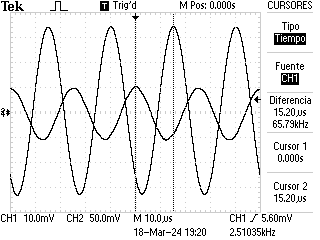
\includegraphics[width=375px]{s1_cap.png}
  \end{center}
  \caption{Captura de l'osci\l.loscopi}
  \label{fig:f1}
\end{figure*}

\newpage

\newthought{Qüestió L2.3: } Veure la taula \ref{tab:t2} i la figura \ref{fig:f2}.

\begin{table}[h]
  \begin{center}
    \begin{tabular}{@{}rccccccccc@{}}
      \toprule
      Freqüència & \qty{0.1}{\kilo\hertz} & \qty{1}{\kilo\hertz} & \qty{10}{\kilo\hertz} & \qty{25}{\kilo\hertz} & \qty{40}{\kilo\hertz} & \qty{75}{\kilo\hertz} & \qty{100}{\kilo\hertz} & \qty{500}{\kilo\hertz} & \qty{1}{\mega\hertz} \\
      \midrule
      $V_i$ &  \qty{10}{\milli\volt} & \qty{10}{\milli\volt} & \qty{10}{\milli\volt} & \qty{10}{\milli\volt} & \qty{10}{\milli\volt} & \qty{10}{\milli\volt} & \qty{10}{\milli\volt} & \qty{10}{\milli\volt} & \qty{10}{\milli\volt} \\
      \midrule
      $V_o$ & \qty{54}{\milli\volt} & \qty{200}{\milli\volt} & \qty{200}{\milli\volt} & \qty{196}{\milli\volt} & \qty{180}{\milli\volt} & \qty{124}{\milli\volt} & \qty{102}{\milli\volt} & \qty{25}{\milli\volt} & \qty{13}{\milli\volt} \\
      \midrule
      Guany & \num{5.4} & \num{20} & \num{20} & \num{19.6} & \num{18} & \num{12.4} & \num{10.2} & \num{2.5} & \num{1.3} \\
      \midrule
      Guany${}_{dB}$ & \qty{33.72}{\deci\bel} & \qty{59.91}{\deci\bel} & \qty{59.91}{\deci\bel} & \qty{59.51}{\deci\bel} & \qty{57.8}{\deci\bel} & \qty{50.35}{\deci\bel} & \qty{46.44}{\deci\bel} & \qty{18.32}{\deci\bel} & \qty{5.24}{\deci\bel} \\
      \bottomrule
    \end{tabular}
  \end{center}
  \caption{Guanys per freqüència}
  \label{tab:t2}
\end{table}

\begin{figure*}[h]
  \begin{center}
    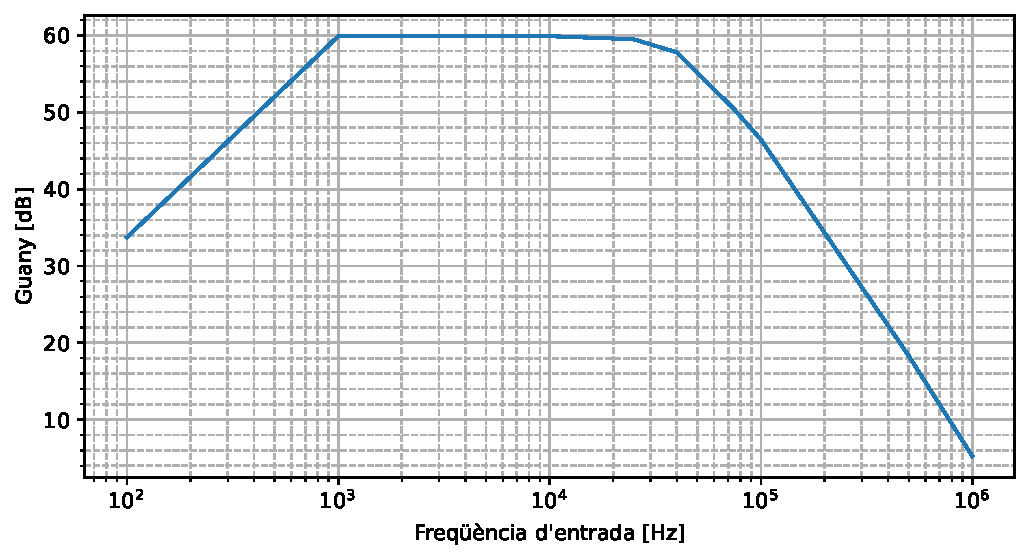
\includegraphics[width=450px]{s1_graph.pdf}
  \end{center}
  \caption{Diagrama de Bode mesurat}
  \label{fig:f2}
\end{figure*}

\newpage

\part{Segona sessió}

\newthought{Qüestió L3.1: } Els nodes $V_{o1}$ i $V_{o2}$ valen \qty{6}{\volt}.
\newthought{Qüestió L3.2: } El guany a la primera etapa val \num{20}, a la segona \num{16.9}. El guany complet val \num{338}. No és el valor desitjat, el muntatge en la protoboard és insuficient.
\newthought{Qüestió L3.3: } Veure la taula \ref{tab:t3} i la figura \ref{fig:f3}. Un altre cop, el muntatge és sorollós.

\begin{table}[h]
  \begin{center}
    \begin{tabular}{@{}rccccccccc@{}}
      \toprule
      Freqüència & \qty{0.1}{\kilo\hertz} & \qty{1}{\kilo\hertz} & \qty{10}{\kilo\hertz} & \qty{25}{\kilo\hertz} & \qty{40}{\kilo\hertz} & \qty{75}{\kilo\hertz} & \qty{100}{\kilo\hertz} & \qty{500}{\kilo\hertz} & \qty{1}{\mega\hertz} \\
      \midrule
      $V_i$ & \qty{10.0}{\milli\volt} & \qty{10.0}{\milli\volt} & \qty{10.0}{\milli\volt} & \qty{10.0}{\milli\volt} & \qty{10.0}{\milli\volt} & \qty{10.0}{\milli\volt} & \qty{10.0}{\milli\volt} & \qty{10.0}{\milli\volt} & \qty{10.0}{\milli\volt} \\
      \midrule
      $V_o$ & \qty{0.25}{\volt} & \qty{3.72}{\volt} & \qty{4.32}{\volt} & \qty{3.34}{\volt} & \qty{1.82}{\volt} & \qty{1.21}{\volt} & \qty{0.05}{\volt} & \qty{0.01}{\volt} & \qty{0.0}{\volt} \\
      \midrule
      Guany & \num{12.8} & \num{186.0} & \num{216.0} & \num{167.0} & \num{91.0} & \num{60.5} & \num{2.75} & \num{0.54} & \num{0.2} \\
      \midrule
      Guany${}_{dB}$ & \qty{32.42}{\deci\bel} & \qty{59.18}{\deci\bel} & \qty{60.68}{\deci\bel} & \qty{58.11}{\deci\bel} & \qty{52.04}{\deci\bel} & \qty{47.95}{\deci\bel} & \qty{17.04}{\deci\bel} & \qty{0.95}{\deci\bel} & \qty{-9.16}{\deci\bel} \\
      \bottomrule
    \end{tabular}
  \end{center}
  \caption{Guanys per freqüència}
  \label{tab:t3}
\end{table}

\begin{figure*}[h]
  \begin{center}
    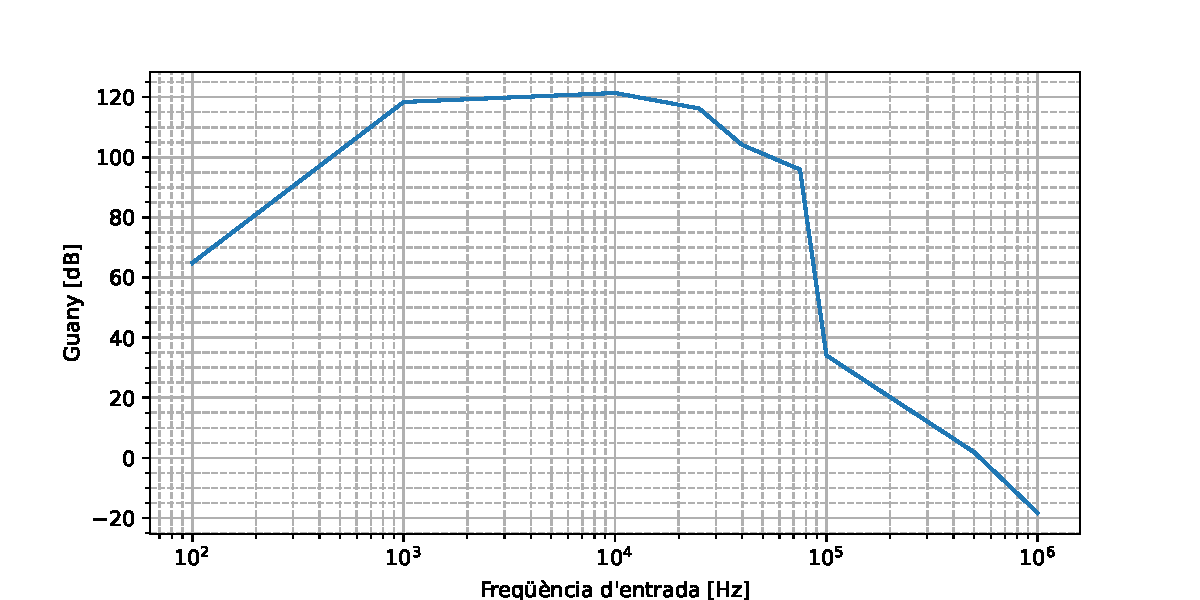
\includegraphics[width=450px]{s2_graph.pdf}
  \end{center}
  \caption{Diagrama de Bode mesurat}
  \label{fig:f3}
\end{figure*}

\newthought{Qüestió L3.4: } La amplitud màxima d'entrada sense distorsió a la sortida és \qty{16.6}{\milli\volt}. Veure la figura \ref{fig:f4}.
\newthought{Qüestió L3.5: } En una variació $\Delta t = \qty{660}{\nano\second}$ hi ha una variació $\Delta V = \qty{11.1}{\volt}$. El SR val \qty{16.8}{\volt\per\micro\second}. Veure la figura \ref{fig:f5}.
\newthought{Qüestió L3.6: } Veure la figura \ref{fig:f6}.

\newpage

\begin{figure}[h]
  \begin{center}
    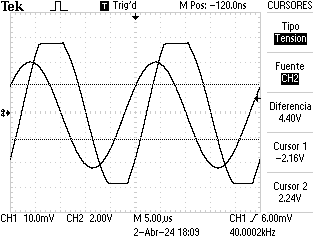
\includegraphics[width=250px]{P4S2_2.png}
  \end{center}
  \caption{Sortida deformada}
  \label{fig:f4}
\end{figure}

\begin{figure}[h]
  \begin{center}
    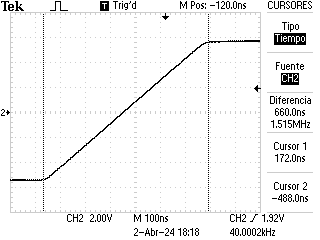
\includegraphics[width=250px]{P4S2_3.png}
  \end{center}
  \caption{Mesura del SR}
  \label{fig:f5}
\end{figure}

\begin{figure*}[!h]
  \begin{center}
    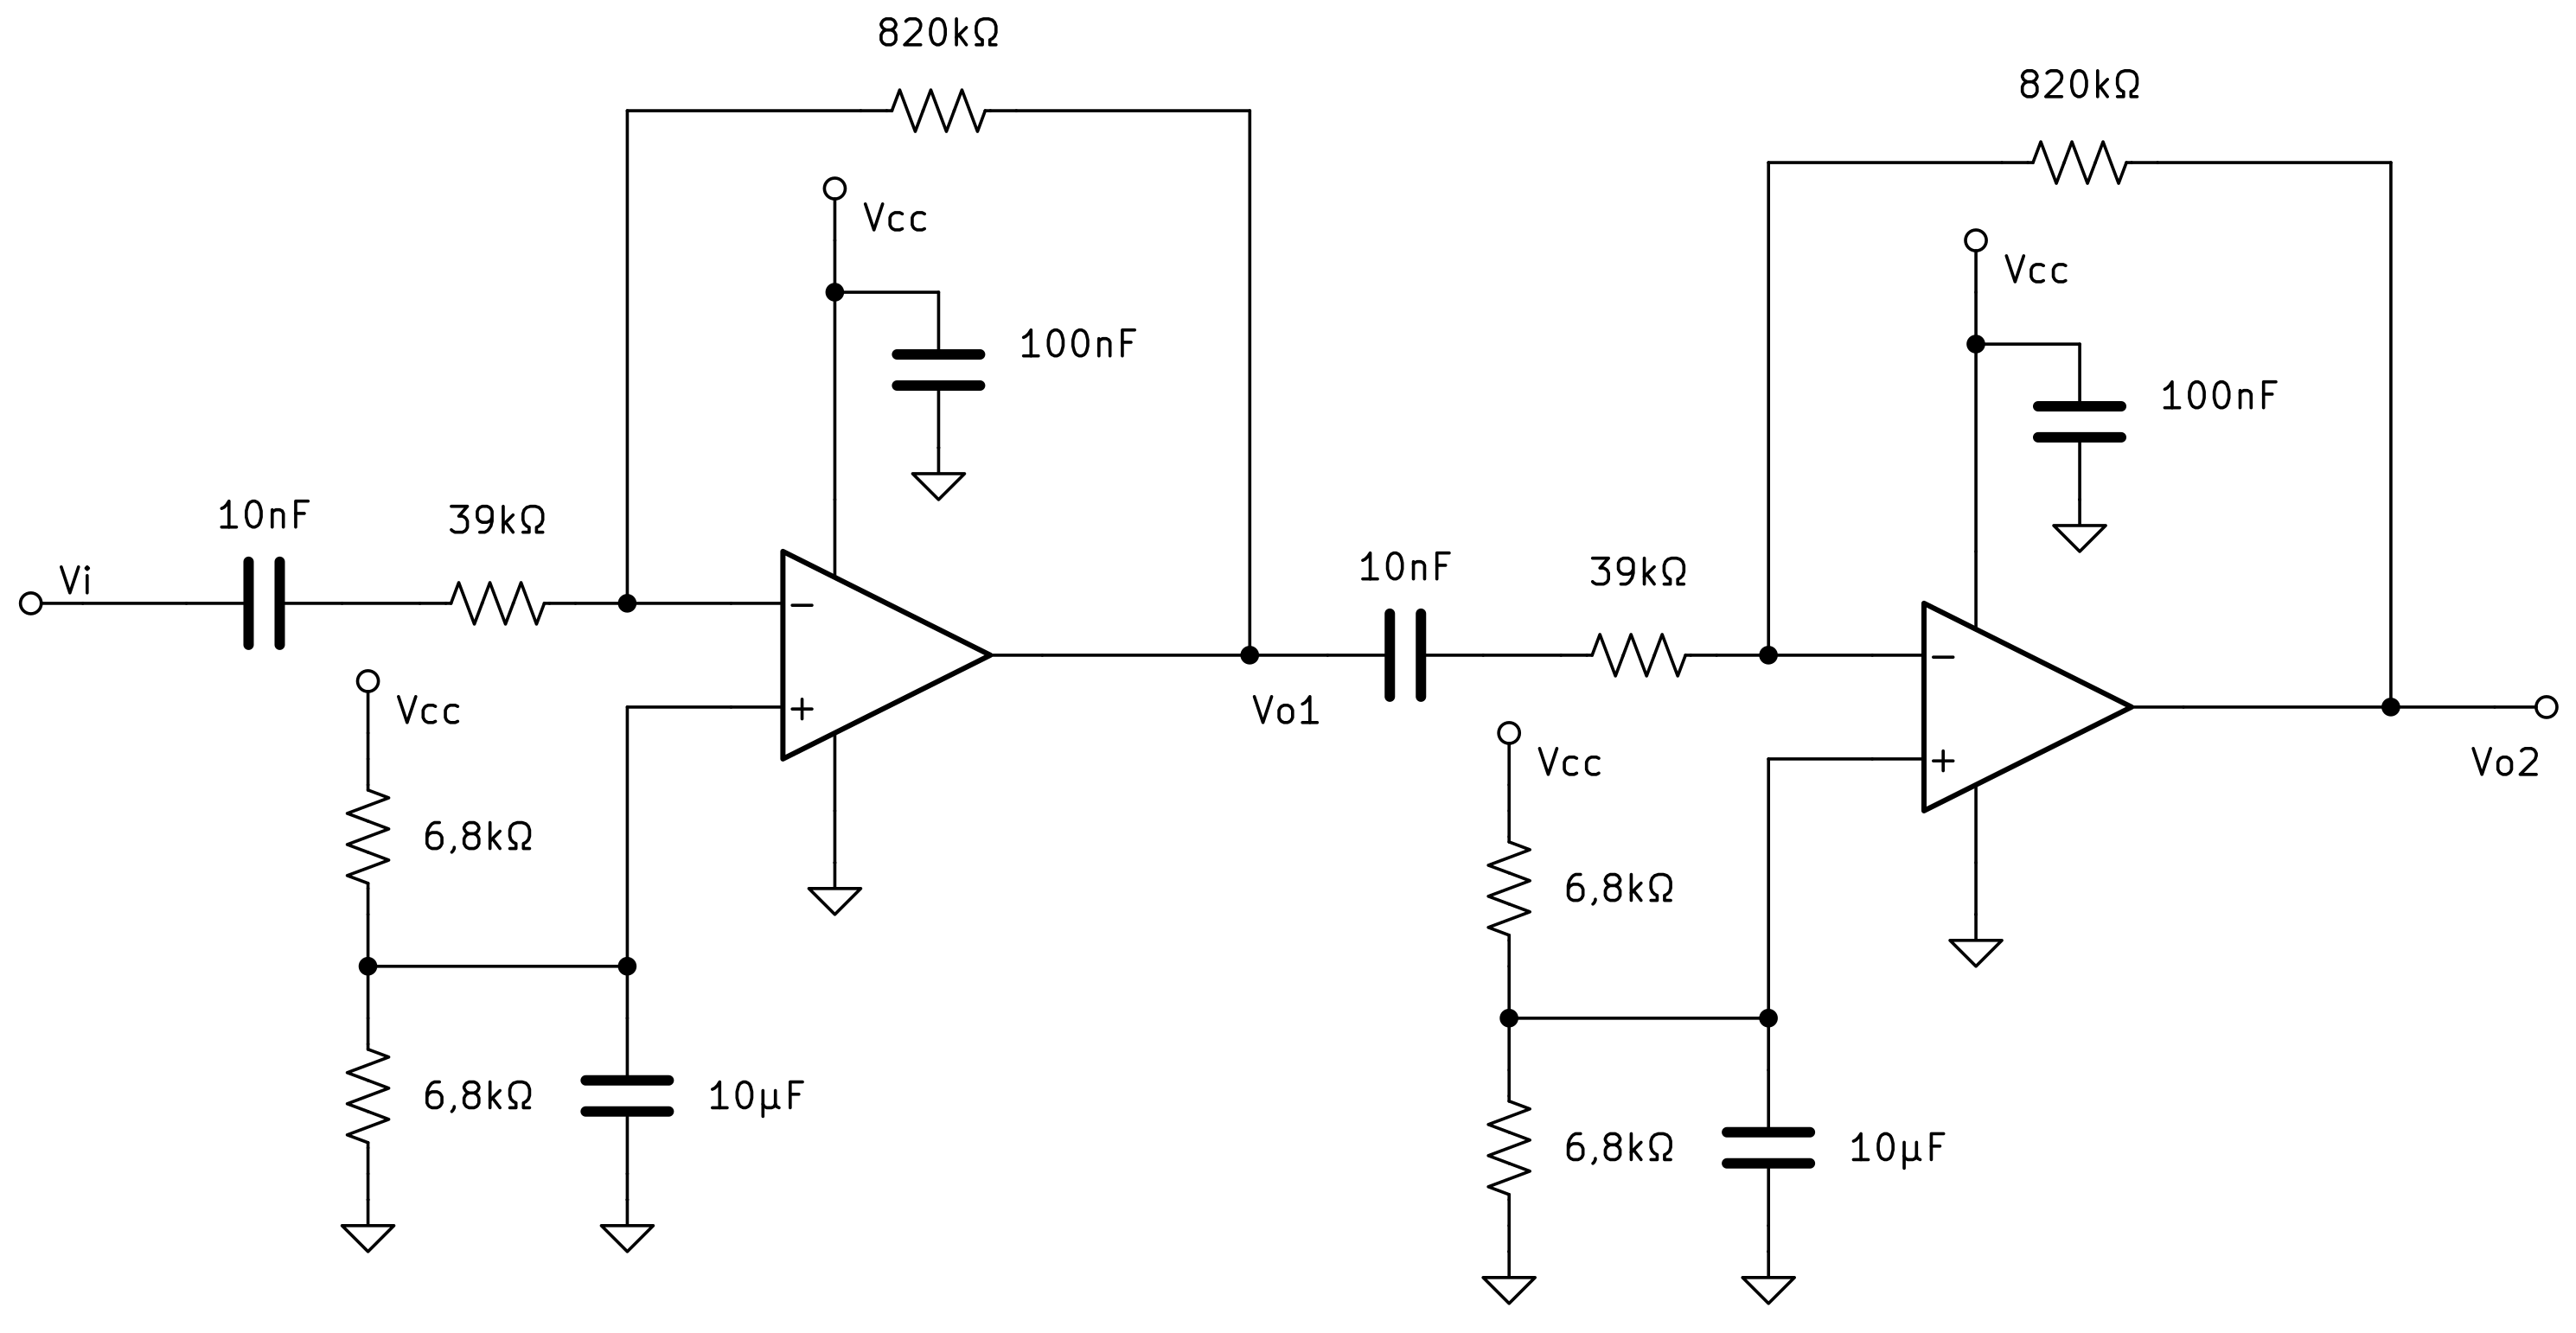
\includegraphics[width=390px]{S2circ.png}
  \end{center}
  \caption{Muntatge complet de les dues etapes}
  \label{fig:f6}
\end{figure*}

\newpage

\part{Tercera sessió}

\newthought{Qüestió L4.1: } El guany de la primera etapa son els \num{20} deistjats.

\begin{figure}[h]
  \begin{center}
    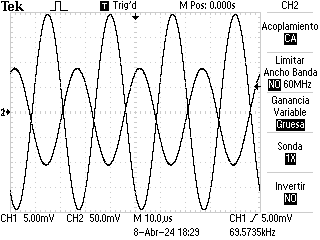
\includegraphics[width=300px]{P4S3_2.png}
  \end{center}
  \caption{Sortida a primera etapa}
\end{figure}

\newthought{Qüestió L4.2: } El guany del muntatge complet val \num{412} i és molt menys sorollós que el muntatge fet en la protoboard.

\begin{figure}[h]
  \begin{center}
    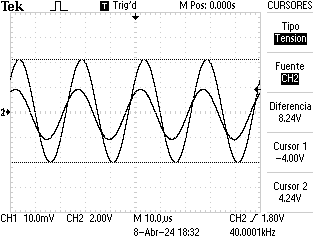
\includegraphics[width=300px]{P4S3_1.png}
  \end{center}
  \caption{Sortida del muntatge complet}
\end{figure}

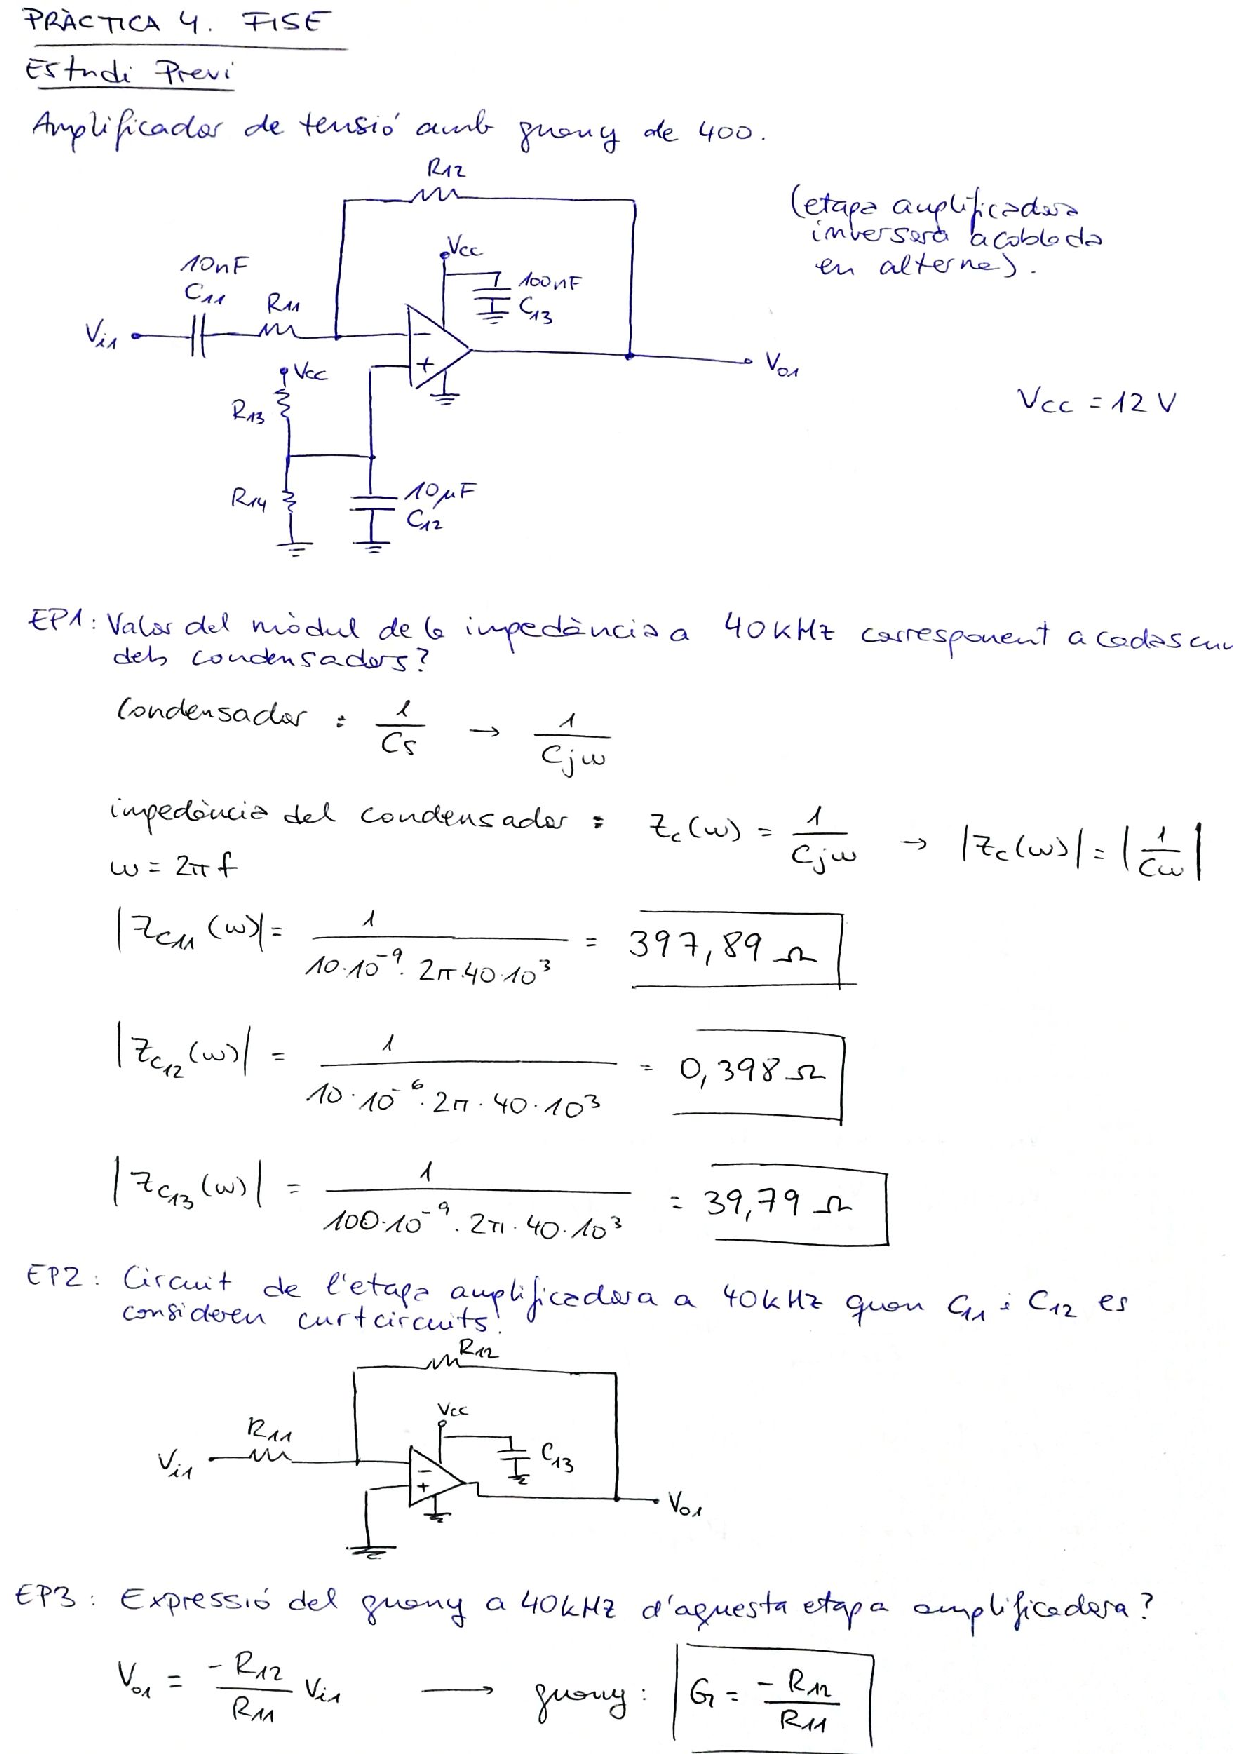
\includepdf[pages={1-4}]{fise_ep_p4.pdf}

\end{document}